\documentclass[aspectratio=169]{beamer}
\usetheme{Madrid}
\usecolortheme{default}

\usepackage{graphicx}
\usepackage{listings}
\usepackage{xcolor}
\usepackage{amsmath}
\usepackage{tikz}

\usepackage{url}

% Code listing setup
\lstset{
    basicstyle=\ttfamily\footnotesize,
    keywordstyle=\color{blue}\bfseries,
    commentstyle=\color{green!60!black},
    stringstyle=\color{red},
    breaklines=true,
    frame=single,
    backgroundcolor=\color{gray!10},
    language=Python
}

\title{The Bootstrap Method}
\subtitle{Resampling for Statistical Inference}
\author{CSE255 - Scalable Data Analysis}
\date{\today}

\begin{document}

\frame{\titlepage}

\begin{frame}{The Problem: Unknown Sampling Distribution}
\small
\begin{itemize}
    \item Traditional statistics assumes known distributions or large samples
    \item What if we have / want to use small sample?
    \item Need a method that doesn't rely on distributional assumptions
    \end{itemize}

\vspace{0.3cm}
\begin{center}
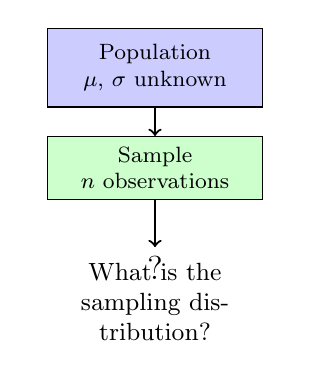
\begin{tikzpicture}[scale=0.85, every node/.style={font=\footnotesize}]
    % Population
    \node[draw, rectangle, fill=blue!20, text width=2.5cm, align=center, minimum height=1cm] (pop) at (0,2.5) {Population\\$\mu$, $\sigma$ unknown};
    
    % Sample
    \node[draw, rectangle, fill=green!20, text width=2.5cm, align=center, minimum height=0.8cm] (sample) at (0,1) {Sample\\$n$ observations};
    
    % Question mark
    \node[text width=3cm, align=center, font=\large] (question) at (0,-0.5) {?};
    \node[text width=3cm, align=center, font=\small] at (0,-1) {What is the\\sampling distribution?};
    
    % Arrow
    \draw[->, thick] (pop) -- (sample);
    \draw[->, thick] (sample) -- (question);
\end{tikzpicture}
\end{center}
\end{frame}

\begin{frame}{What is Bootstrap?}
\footnotesize
\textbf{Definition:}
\begin{itemize}
    \item Resampling with replacement from observed data
    \item Treat the sample as if it were the population
    \item Created by Bradley Efron (1979)
    \item Non-parametric method
\end{itemize}

\vspace{0.2cm}
\textbf{Key Idea:}
\begin{itemize}
    \item If the sample is representative, resampling from it approximates resampling from the population
    \item Bootstrap distribution approximates the sampling distribution
    \item No distributional assumptions needed
\end{itemize}

\vspace{0.15cm}
\textbf{Advantages:}
\begin{itemize}
    \item Works with any sample size
    \item Works with any statistic
    \item Works with complex distributions
\end{itemize}
\end{frame}

\begin{frame}{Bootstrap Procedure: Step-by-Step}
\scriptsize
\textbf{The Bootstrap Algorithm:}

\begin{enumerate}
    \item \textbf{Start} with original sample of size $n$: $X = \{x_1, x_2, \ldots, x_n\}$
    \item \textbf{Draw} $n$ observations with replacement (bootstrap sample): $X^*_1$
    \item \textbf{Compute} statistic of interest on bootstrap sample: $\theta^*_1 = T(X^*_1)$
    \item \textbf{Repeat} steps 2-3 $B$ times (typically 1000-10000): $X^*_2, X^*_3, \ldots, X^*_B$
    \item \textbf{Use} distribution of bootstrap statistics $\{\theta^*_1, \theta^*_2, \ldots, \theta^*_B\}$ for inference
\end{enumerate}

\vspace{0.1cm}
\begin{center}
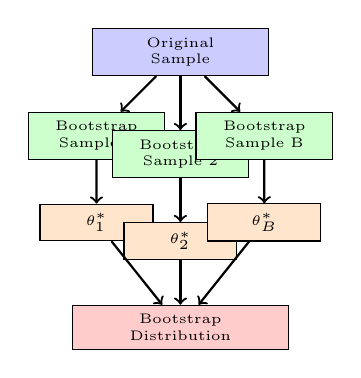
\begin{tikzpicture}[node distance=0.8cm, auto, scale=0.65, every node/.style={font=\tiny}]
    % Original sample
    \node[draw, rectangle, fill=blue!20, text width=2cm, align=center] (orig) {Original\\Sample};
    
    % Bootstrap samples
    \node[draw, rectangle, fill=green!20, text width=1.5cm, align=center, below left of=orig, xshift=-0.5cm, yshift=-0.5cm] (b1) {Bootstrap\\Sample 1};
    \node[draw, rectangle, fill=green!20, text width=1.5cm, align=center, below of=orig, yshift=-0.5cm] (b2) {Bootstrap\\Sample 2};
    \node[draw, rectangle, fill=green!20, text width=1.5cm, align=center, below right of=orig, xshift=0.5cm, yshift=-0.5cm] (b3) {Bootstrap\\Sample B};
    
    % Statistics
    \node[draw, rectangle, fill=orange!20, text width=1.2cm, align=center, below of=b1, yshift=-0.3cm] (s1) {$\theta^*_1$};
    \node[draw, rectangle, fill=orange!20, text width=1.2cm, align=center, below of=b2, yshift=-0.3cm] (s2) {$\theta^*_2$};
    \node[draw, rectangle, fill=orange!20, text width=1.2cm, align=center, below of=b3, yshift=-0.3cm] (s3) {$\theta^*_B$};
    
    % Distribution
    \node[draw, rectangle, fill=red!20, text width=2.5cm, align=center, below of=s2, yshift=-0.3cm] (dist) {Bootstrap\\Distribution};
    
    % Arrows
    \draw[->, thick] (orig) -- (b1);
    \draw[->, thick] (orig) -- (b2);
    \draw[->, thick] (orig) -- (b3);
    \draw[->, thick] (b1) -- (s1);
    \draw[->, thick] (b2) -- (s2);
    \draw[->, thick] (b3) -- (s3);
    \draw[->, thick] (s1) -- (dist);
    \draw[->, thick] (s2) -- (dist);
    \draw[->, thick] (s3) -- (dist);
\end{tikzpicture}
\end{center}
\end{frame}

\begin{frame}{Bootstrap Resampling: Visual Example}
\scriptsize
\textbf{Original Sample:} $X = [x_1, x_2, x_3, x_4, x_5]$

\vspace{0.1cm}
\begin{center}
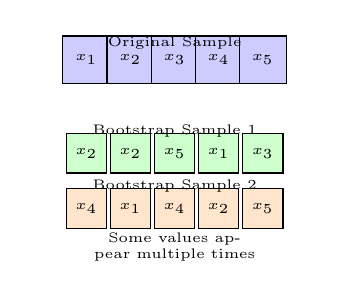
\begin{tikzpicture}[node distance=0.6cm, auto, scale=0.7, every node/.style={font=\tiny}]
    % Original sample boxes
    \foreach \i/\val in {1/1, 2/2, 3/3, 4/4, 5/5} {
        \node[draw, rectangle, fill=blue!20, minimum width=0.6cm, minimum height=0.6cm] (orig\i) at (\i*0.8, 2) {$x_{\val}$};
    }
    \node[font=\tiny] at (2.4, 2.3) {Original Sample};
    
    % Bootstrap sample 1
    \node[draw, rectangle, fill=green!20, minimum width=0.5cm, minimum height=0.5cm] (b1_1) at (0.8, 0.3) {$x_2$};
    \node[draw, rectangle, fill=green!20, minimum width=0.5cm, minimum height=0.5cm] (b1_2) at (1.6, 0.3) {$x_2$};
    \node[draw, rectangle, fill=green!20, minimum width=0.5cm, minimum height=0.5cm] (b1_3) at (2.4, 0.3) {$x_5$};
    \node[draw, rectangle, fill=green!20, minimum width=0.5cm, minimum height=0.5cm] (b1_4) at (3.2, 0.3) {$x_1$};
    \node[draw, rectangle, fill=green!20, minimum width=0.5cm, minimum height=0.5cm] (b1_5) at (4.0, 0.3) {$x_3$};
    \node[font=\tiny] at (2.4, 0.7) {Bootstrap Sample 1};
    
    % Bootstrap sample 2
    \node[draw, rectangle, fill=orange!20, minimum width=0.5cm, minimum height=0.5cm] (b2_1) at (0.8, -0.7) {$x_4$};
    \node[draw, rectangle, fill=orange!20, minimum width=0.5cm, minimum height=0.5cm] (b2_2) at (1.6, -0.7) {$x_1$};
    \node[draw, rectangle, fill=orange!20, minimum width=0.5cm, minimum height=0.5cm] (b2_3) at (2.4, -0.7) {$x_4$};
    \node[draw, rectangle, fill=orange!20, minimum width=0.5cm, minimum height=0.5cm] (b2_4) at (3.2, -0.7) {$x_2$};
    \node[draw, rectangle, fill=orange!20, minimum width=0.5cm, minimum height=0.5cm] (b2_5) at (4.0, -0.7) {$x_5$};
    \node[font=\tiny] at (2.4, -0.3) {Bootstrap Sample 2};
    
    % Note
    \node[font=\tiny, text width=3.5cm, align=center] at (2.4, -1.4) {Some values appear multiple times};
\end{tikzpicture}
\end{center}
\end{frame}

\begin{frame}{Bootstrap Distribution}
\footnotesize
\textbf{Key Concept:}
\begin{itemize}
    \item The collection of all bootstrap statistics forms the \textbf{bootstrap distribution}
    \item This approximates the \textbf{sampling distribution} of the statistic
    \item Bootstrap distribution $\approx$ Sampling distribution
\end{itemize}

\vspace{0.1cm}
\begin{center}
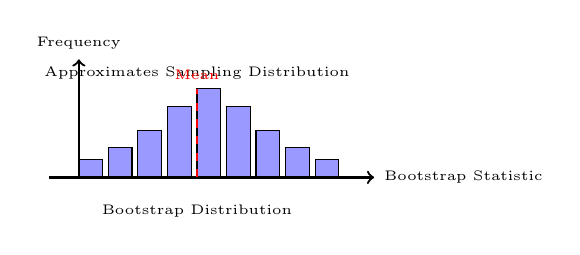
\begin{tikzpicture}[scale=0.75, every node/.style={font=\tiny}]
    % Histogram bars
    \foreach \x/\h in {0/0.3, 0.5/0.5, 1/0.8, 1.5/1.2, 2/1.5, 2.5/1.2, 3/0.8, 3.5/0.5, 4/0.3} {
        \draw[fill=blue!40] (\x, 0) rectangle (\x+0.4, \h);
    }
    
    % Axes
    \draw[->, thick] (-0.5, 0) -- (5, 0) node[right] {Bootstrap Statistic};
    \draw[->, thick] (0, 0) -- (0, 2) node[above] {Frequency};
    
    % Labels
    \node[below, font=\tiny] at (2, -0.3) {Bootstrap Distribution};
    \node[above, font=\tiny] at (2, 1.5) {Approximates Sampling Distribution};
    
    % Mean marker
    \draw[dashed, thick, red] (2, 0) -- (2, 1.5);
    \node[red, above, font=\tiny] at (2, 1.5) {Mean};
\end{tikzpicture}
\end{center}

\vspace{0.05cm}
\textbf{Properties:}
\begin{itemize}
    \item Bootstrap distribution is centered around the sample statistic
    \item Spread reflects uncertainty in the statistic
    \item Can be used for confidence intervals, hypothesis tests, etc.
\end{itemize}
\end{frame}

\begin{frame}{Bootstrap Confidence Intervals: Percentile Method}
\scriptsize
\textbf{Percentile Method:}
\begin{enumerate}
    \item Sort bootstrap statistics: $\theta^*_{(1)} \leq \theta^*_{(2)} \leq \ldots \leq \theta^*_{(B)}$
    \item Take percentiles for $(1-\alpha)$ confidence interval
    \item For 95\% CI: $[\theta^*_{(0.025B)}, \theta^*_{(0.975B)}]$
\end{enumerate}

\vspace{0.1cm}
\textbf{Formula:}
\[
CI_{1-\alpha} = [\theta^*_{(\alpha/2)}, \theta^*_{(1-\alpha/2)}]
\]

\vspace{0.1cm}
\begin{center}
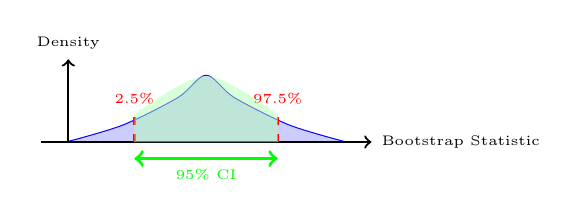
\begin{tikzpicture}[scale=0.7, every node/.style={font=\tiny}]
    % Distribution curve
    \draw[thick, blue] plot[smooth] coordinates {(0,0) (1,0.3) (2,0.8) (2.5,1.2) (3,0.8) (4,0.3) (5,0)};
    \fill[blue!20] plot[smooth] coordinates {(0,0) (1,0.3) (2,0.8) (2.5,1.2) (3,0.8) (4,0.3) (5,0)} -- (5,0) -- (0,0);
    
    % Axes
    \draw[->, thick] (-0.5, 0) -- (5.5, 0) node[right] {Bootstrap Statistic};
    \draw[->, thick] (0, 0) -- (0, 1.5) node[above] {Density};
    
    % Percentile markers
    \draw[dashed, thick, red] (1.2, 0) -- (1.2, 0.5) node[above, font=\tiny] {2.5\%};
    \draw[dashed, thick, red] (3.8, 0) -- (3.8, 0.5) node[above, font=\tiny] {97.5\%};
    
    % Confidence interval
    \draw[<->, very thick, green] (1.2, -0.3) -- (3.8, -0.3) node[midway, below, font=\tiny] {95\% CI};
    
    % Shaded region
    \fill[green!30, opacity=0.5] (1.2, 0) -- plot[smooth] coordinates {(1.2,0.5) (2.5,1.2) (3.8,0.5)} -- (3.8, 0) -- cycle;
\end{tikzpicture}
\end{center}
\end{frame}

\begin{frame}[fragile]{Bootstrap Confidence Intervals: Code Example}
\scriptsize
\textbf{Python Implementation:}
\begin{lstlisting}[basicstyle=\tiny]
import numpy as np

# Original sample
data = np.array([1.2, 2.5, 3.1, 4.0, 5.2, 6.3, 7.1])
n = len(data)
B = 10000  # Number of bootstrap samples

# Bootstrap resampling
bootstrap_means = []
for i in range(B):
    bootstrap_sample = np.random.choice(data, size=n, replace=True)
    bootstrap_means.append(np.mean(bootstrap_sample))

# Compute 95% confidence interval
ci_lower = np.percentile(bootstrap_means, 2.5)
ci_upper = np.percentile(bootstrap_means, 97.5)
print(f"95% CI: [{ci_lower:.3f}, {ci_upper:.3f}]")
\end{lstlisting}

\vspace{0.03cm}
\textbf{Using scipy.stats.bootstrap:}
\begin{lstlisting}[basicstyle=\tiny]
from scipy.stats import bootstrap

result = bootstrap((data,), np.mean, 
                  confidence_level=0.95, 
                  n_resamples=10000)
print(f"95% CI: [{result.confidence_interval.low:.3f}, "
      f"{result.confidence_interval.high:.3f}]")
\end{lstlisting}
\end{frame}

\begin{frame}{Bootstrap vs. Traditional Methods}
\scriptsize
\begin{center}
\begin{tabular}{|l|p{3cm}|p{3cm}|}
\hline
\textbf{Aspect} & \textbf{Bootstrap} & \textbf{Traditional} \\
\hline
\textbf{Assumptions} & Minimal (i.i.d.) & Distributional \\
\hline
\textbf{Sample Size} & Any size & Large $n$ preferred \\
\hline
\textbf{Complexity} & Computational & Analytical \\
\hline
\textbf{Accuracy} & Good approximation & Exact if assumptions hold \\
\hline
\textbf{Flexibility} & Any statistic & Limited formulas \\
\hline
\textbf{Computation} & Intensive & Fast \\
\hline
\end{tabular}
\end{center}

\vspace{0.1cm}
\textbf{When Bootstrap Wins:}
\begin{itemize}
    \item Small samples
    \item Non-standard statistics
    \item Unknown distributions
    \item Difficult analytical solutions
\end{itemize}

\vspace{0.05cm}
\textbf{When Traditional Wins:}
\begin{itemize}
    \item Large samples, known distributions
    \item Standard statistics
    \item Need for speed
\end{itemize}
\end{frame}

\begin{frame}{When to Use Bootstrap}
\footnotesize
\textbf{Use Bootstrap When:}
\begin{itemize}
    \item \textbf{Small sample sizes} - Traditional methods may not apply
    \item \textbf{Unknown or complex distributions} - No distributional assumptions needed
    \item \textbf{Non-standard statistics} - Median, trimmed mean, robust estimators
    \item \textbf{Analytical solutions are difficult} - Complex estimators
    \item \textbf{Validating other methods} - Check if assumptions are reasonable
    \item \textbf{Confidence intervals for any statistic} - Not just mean/variance
\end{itemize}

\vspace{0.2cm}
\textbf{Example Scenarios:}
\begin{itemize}
    \item Confidence interval for median income
    \item Standard error of correlation coefficient
    \item Confidence interval for regression coefficients
    \item Hypothesis testing with non-normal data
    \item Quantile estimation
\end{itemize}
\end{frame}

\begin{frame}{Bootstrap Hypothesis Testing}
\scriptsize
\textbf{Procedure:}
\begin{enumerate}
    \item Generate bootstrap distribution under null hypothesis $H_0$
    \item Compare observed statistic to bootstrap distribution
    \item Compute p-value from bootstrap distribution
\end{enumerate}

\vspace{0.1cm}
\textbf{Example: Testing if mean equals $\mu_0$}
\begin{itemize}
    \item $H_0: \mu = \mu_0$ vs. $H_1: \mu \neq \mu_0$
    \item Center bootstrap samples at $\mu_0$: $X^* - \bar{X} + \mu_0$
    \item Compute bootstrap distribution of means
    \item p-value = proportion of bootstrap means as extreme as observed
\end{itemize}

\vspace{0.1cm}
\begin{center}
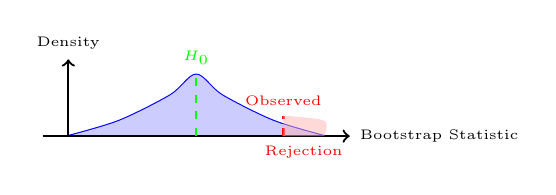
\begin{tikzpicture}[scale=0.65, every node/.style={font=\tiny}]
    % Distribution curve
    \draw[thick, blue] plot[smooth] coordinates {(0,0) (1,0.3) (2,0.8) (2.5,1.2) (3,0.8) (4,0.3) (5,0)};
    \fill[blue!20] plot[smooth] coordinates {(0,0) (1,0.3) (2,0.8) (2.5,1.2) (3,0.8) (4,0.3) (5,0)} -- (5,0) -- (0,0);
    
    % Axes
    \draw[->, thick] (-0.5, 0) -- (5.5, 0) node[right] {Bootstrap Statistic};
    \draw[->, thick] (0, 0) -- (0, 1.5) node[above] {Density};
    
    % Observed value
    \draw[dashed, very thick, red] (4.2, 0) -- (4.2, 0.4);
    \node[red, above, font=\tiny] at (4.2, 0.4) {Observed};
    
    % Rejection region
    \fill[red!30, opacity=0.5] (4.2, 0) -- plot[smooth] coordinates {(4.2,0.4) (5,0.3) (5,0)} -- (4.2, 0) -- cycle;
    \node[red, below, font=\tiny] at (4.6, 0) {Rejection};
    
    % Null value
    \draw[dashed, thick, green] (2.5, 0) -- (2.5, 1.2);
    \node[green, above, font=\tiny] at (2.5, 1.2) {$H_0$};
\end{tikzpicture}
\end{center}
\end{frame}

\begin{frame}{Bootstrap Applications: Regression}
\footnotesize
\textbf{Bootstrap for Regression:}
\begin{itemize}
    \item \textbf{Case resampling}: Resample entire observations $(x_i, y_i)$
    \item \textbf{Residual resampling}: Resample residuals, keep $x_i$ fixed
    \item Confidence intervals for coefficients
    \item Model validation and diagnostics
\end{itemize}

\vspace{0.1cm}
\textbf{Case Resampling:}
\begin{enumerate}
    \item Resample pairs $(x_i, y_i)$ with replacement
    \item Fit regression model to bootstrap sample
    \item Collect coefficients $\beta^*_1, \beta^*_2, \ldots, \beta^*_B$
    \item Use distribution for inference
\end{enumerate}

\vspace{0.1cm}
\textbf{Residual Resampling:}
\begin{enumerate}
    \item Fit model, get residuals $e_i = y_i - \hat{y}_i$
    \item Resample residuals: $e^*_i$
    \item Create bootstrap response: $y^*_i = \hat{y}_i + e^*_i$
    \item Refit model, collect coefficients
\end{enumerate}

\vspace{0.05cm}
\textbf{Use Case:} CI for coefficients when errors are non-normal
\end{frame}

\begin{frame}{Bootstrap Applications: Time Series}
\footnotesize
\textbf{Challenge:} Standard bootstrap assumes independence

\vspace{0.1cm}
\textbf{Block Bootstrap:}
\begin{itemize}
    \item Preserves temporal structure
    \item Resample blocks of consecutive observations
    \item Maintains dependence within blocks
    \item Useful for time series, spatial data
\end{itemize}

\vspace{0.1cm}
\textbf{Procedure:}
\begin{enumerate}
    \item Divide time series into blocks of length $l$
    \item Resample blocks with replacement
    \item Concatenate blocks to form bootstrap series
    \item Compute statistic on bootstrap series
\end{enumerate}

\vspace{0.1cm}
\textbf{Example:}
\begin{itemize}
    \item Original: $[x_1, x_2, x_3, x_4, x_5, x_6]$
    \item Blocks: $[x_1, x_2]$, $[x_3, x_4]$, $[x_5, x_6]$
    \item Bootstrap: $[x_3, x_4, x_1, x_2, x_5, x_6]$
\end{itemize}

\vspace{0.05cm}
\textbf{Note:} Block length $l$ must be chosen carefully
\end{frame}

\begin{frame}{Computational Considerations}
\footnotesize
\textbf{Computational Cost:}
\begin{itemize}
    \item Bootstrap requires many resamples (typically 1000-10000)
    \item Each resample requires computing the statistic
    \item Can be computationally intensive for large datasets
\end{itemize}

\vspace{0.1cm}
\textbf{Speedup Strategies:}
\begin{itemize}
    \item \textbf{Parallel computing}: Resamples are independent
    \item \textbf{Vectorization}: Use NumPy operations
    \item \textbf{Reduced resamples}: Use fewer for rough estimates
    \item \textbf{Smart sampling}: Adaptive resampling strategies
\end{itemize}

\vspace{0.1cm}
\textbf{Connection to Scalable Data Analysis:}
\begin{itemize}
    \item Bootstrap is embarrassingly parallel
    \item Each resample can be computed independently
    \item Perfect for distributed computing (Dask, Spark)
    \item Trade-off: More resamples = better accuracy but more computation
\end{itemize}

\vspace{0.05cm}
\textbf{Rule of Thumb:} Use at least 1000 resamples for 95\% CI
\end{frame}

\begin{frame}{Bootstrap Limitations}
\scriptsize
\textbf{Important Limitations:}
\begin{itemize}
    \item \textbf{Requires independent observations} (or block bootstrap)
    \item \textbf{May not work well for very small samples} ($n < 10$)
    \item \textbf{Can be computationally expensive} for large datasets
    \item \textbf{Not a panacea} - still requires careful application
    \item \textbf{Bias issues} - Bootstrap can be biased for some statistics
    \item \textbf{Edge cases} - May fail for statistics near boundaries
\end{itemize}

\vspace{0.05cm}
\textbf{When Bootstrap Fails:}
\begin{itemize}
    \item Dependent data (without block bootstrap)
    \item Very small samples
    \item Heavy-tailed distributions
    \item Statistics that are not smooth functions of data
\end{itemize}

\vspace{0.05cm}
\textbf{Best Practices:}
\begin{itemize}
    \item Check assumptions (independence, representativeness)
    \item Use appropriate number of resamples
    \item Consider bias-corrected methods if needed
    \item Validate with known examples
\end{itemize}
\end{frame}

\begin{frame}{Bootstrap Variants}
\scriptsize
\textbf{1. Parametric Bootstrap:}
\begin{itemize}
    \item Assume a parametric model (e.g., normal)
    \item Estimate parameters from data
    \item Resample from fitted model
    \item More efficient if model is correct
\end{itemize}

\vspace{0.05cm}
\textbf{2. Smoothed Bootstrap:}
\begin{itemize}
    \item Add small random noise to resampled values
    \item Smooths the bootstrap distribution
    \item Useful for continuous data
\end{itemize}

\vspace{0.05cm}
\textbf{3. Wild Bootstrap:}
\begin{itemize}
    \item For heteroscedastic regression
    \item Resample residuals with random weights
    \item Preserves heteroscedasticity structure
\end{itemize}

\vspace{0.05cm}
\textbf{4. Block Bootstrap:}
\begin{itemize}
    \item For dependent data (time series, spatial)
    \item Resample blocks instead of individual observations
    \item Preserves dependence structure
\end{itemize}

\vspace{0.05cm}
\textbf{5. Bias-Corrected and Accelerated (BCa):}
\begin{itemize}
    \item Adjusts for bias and skewness
    \item More accurate confidence intervals
    \item Requires estimating acceleration parameter
\end{itemize}
\end{frame}

\begin{frame}{Bagging: Bootstrap Aggregating}
\footnotesize
\textbf{What is Bagging?}
\begin{itemize}
    \item \textbf{Bagging} = \textbf{B}ootstrap \textbf{Agg}regat\textbf{ing}
    \item Machine learning technique that uses bootstrap sampling
    \item Created by Leo Breiman (1996)
    \item Reduces variance and improves model stability
\end{itemize}

\vspace{0.2cm}
\textbf{Key Idea:}
\begin{itemize}
    \item Train multiple models on different bootstrap samples
    \item Aggregate predictions (average for regression, vote for classification)
    \item Reduces overfitting and improves generalization
    \item Works especially well with unstable learners (trees, neural networks)
\end{itemize}

\vspace{0.15cm}
\textbf{Connection to Bootstrap:}
\begin{itemize}
    \item Uses bootstrap sampling to create diverse training sets
    \item Each model sees different subset of data
    \item Ensemble of models is more robust than single model
\end{itemize}
\end{frame}

\begin{frame}{Bagging Algorithm}
\footnotesize
\textbf{The Bagging Procedure:}

\begin{enumerate}
    \item \textbf{For} $b = 1, 2, \ldots, B$:
    \begin{itemize}
        \item Create bootstrap sample $D^*_b$ by sampling $n$ observations with replacement
        \item Train model $f^*_b$ on bootstrap sample $D^*_b$
    \end{itemize}
    \item \textbf{Aggregate} predictions:
    \begin{itemize}
        \item \textbf{Regression}: $\hat{f}_{bag}(x) = \frac{1}{B}\sum_{b=1}^B f^*_b(x)$
        \item \textbf{Classification}: Majority vote of $f^*_1(x), \ldots, f^*_B(x)$
    \end{itemize}
\end{enumerate}

\vspace{0.2cm}
\begin{center}
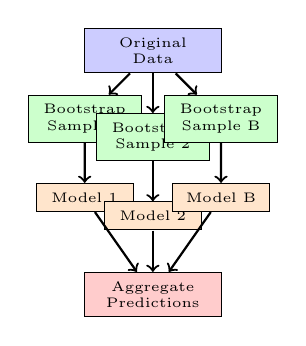
\begin{tikzpicture}[node distance=0.8cm, auto, scale=0.7, every node/.style={font=\tiny}]
    % Original data
    \node[draw, rectangle, fill=blue!20, text width=1.5cm, align=center] (data) {Original\\Data};
    
    % Bootstrap samples
    \node[draw, rectangle, fill=green!20, text width=1.2cm, align=center, below left of=data, xshift=-0.3cm, yshift=-0.3cm] (b1) {Bootstrap\\Sample 1};
    \node[draw, rectangle, fill=green!20, text width=1.2cm, align=center, below of=data, yshift=-0.3cm] (b2) {Bootstrap\\Sample 2};
    \node[draw, rectangle, fill=green!20, text width=1.2cm, align=center, below right of=data, xshift=0.3cm, yshift=-0.3cm] (b3) {Bootstrap\\Sample B};
    
    % Models
    \node[draw, rectangle, fill=orange!20, text width=1cm, align=center, below of=b1, yshift=-0.2cm] (m1) {Model 1};
    \node[draw, rectangle, fill=orange!20, text width=1cm, align=center, below of=b2, yshift=-0.2cm] (m2) {Model 2};
    \node[draw, rectangle, fill=orange!20, text width=1cm, align=center, below of=b3, yshift=-0.2cm] (m3) {Model B};
    
    % Aggregate
    \node[draw, rectangle, fill=red!20, text width=1.5cm, align=center, below of=m2, yshift=-0.2cm] (agg) {Aggregate\\Predictions};
    
    % Arrows
    \draw[->, thick] (data) -- (b1);
    \draw[->, thick] (data) -- (b2);
    \draw[->, thick] (data) -- (b3);
    \draw[->, thick] (b1) -- (m1);
    \draw[->, thick] (b2) -- (m2);
    \draw[->, thick] (b3) -- (m3);
    \draw[->, thick] (m1) -- (agg);
    \draw[->, thick] (m2) -- (agg);
    \draw[->, thick] (m3) -- (agg);
\end{tikzpicture}
\end{center}
\end{frame}

\begin{frame}{Why Bagging Works}
\footnotesize
\textbf{Variance Reduction:}
\begin{itemize}
    \item Single model has high variance (sensitive to training data)
    \item Averaging multiple models reduces variance
    \item Variance of average: $\text{Var}(\bar{X}) = \frac{\text{Var}(X)}{B}$
    \item More models $\rightarrow$ lower variance
\end{itemize}

\vspace{0.15cm}
\textbf{Bias-Variance Trade-off:}
\begin{itemize}
    \item Bagging doesn't change bias (models trained on same distribution)
    \item Reduces variance without increasing bias
    \item Net effect: Lower prediction error
\end{itemize}

\vspace{0.15cm}
\textbf{When Bagging Helps Most:}
\begin{itemize}
    \item Unstable learners (decision trees, neural networks)
    \item High-variance models
    \item When overfitting is a concern
    \item Less effective for stable learners (linear models, k-NN)
\end{itemize}
\end{frame}

\begin{frame}{Random Forests: Bagging + Feature Randomness}
\footnotesize
\textbf{Random Forests:}
\begin{itemize}
    \item Extension of bagging for decision trees
    \item Combines bagging with random feature selection
    \item Each tree uses bootstrap sample AND random subset of features
    \item Further reduces correlation between trees
\end{itemize}

\vspace{0.15cm}
\textbf{Algorithm:}
\begin{enumerate}
    \item For $b = 1, 2, \ldots, B$:
    \begin{itemize}
        \item Create bootstrap sample $D^*_b$
        \item At each split, randomly select $m$ features from $p$ total
        \item Grow tree $T^*_b$ using only these $m$ features
    \end{itemize}
    \item Aggregate predictions from all $B$ trees
\end{enumerate}

\vspace{0.15cm}
\textbf{Key Parameters:}
\begin{itemize}
    \item $B$: Number of trees (typically 100-500)
    \item $m$: Number of features per split (typically $\sqrt{p}$ for classification, $p/3$ for regression)
    \item Tree depth: Usually grown to full depth
\end{itemize}
\end{frame}

\begin{frame}{Bagging vs. Single Model}
\scriptsize
\textbf{Advantages of Bagging:}
\begin{itemize}
    \item \textbf{Lower variance}: More stable predictions
    \item \textbf{Better generalization}: Reduced overfitting
    \item \textbf{Robustness}: Less sensitive to outliers
    \item \textbf{Parallelizable}: Models can be trained independently
    \item \textbf{No additional assumptions}: Works with any base learner
\end{itemize}

\vspace{0.1cm}
\textbf{Disadvantages:}
\begin{itemize}
    \item \textbf{Computational cost}: Need to train $B$ models
    \item \textbf{Memory}: Need to store $B$ models
    \item \textbf{Interpretability}: Harder to interpret ensemble than single model
    \item \textbf{Diminished returns}: Benefits plateau as $B$ increases
\end{itemize}

\vspace{0.05cm}
\textbf{Rule of Thumb:} Use $B = 100$ to $500$ trees. Beyond that, improvements are marginal.
\end{frame}

\begin{frame}[fragile]{Bagging in Python: Example}
\tiny
\textbf{Using sklearn:}
\begin{lstlisting}[basicstyle=\tiny]
from sklearn.ensemble import BaggingClassifier
from sklearn.tree import DecisionTreeClassifier

base_estimator = DecisionTreeClassifier(max_depth=10)
bagging = BaggingClassifier(
    base_estimator=base_estimator,
    n_estimators=100,  # B = 100
    max_samples=1.0,   # Use full bootstrap sample
    bootstrap=True,    # Sample with replacement
    random_state=42
)
bagging.fit(X_train, y_train)
predictions = bagging.predict(X_test)
\end{lstlisting}

\vspace{0.03cm}
\textbf{Random Forest (specialized bagging):}
\begin{lstlisting}[basicstyle=\tiny]
from sklearn.ensemble import RandomForestClassifier

rf = RandomForestClassifier(
    n_estimators=100,
    max_features='sqrt',  # m = sqrt(p)
    random_state=42
)
rf.fit(X_train, y_train)
\end{lstlisting}
\end{frame}

\begin{frame}[fragile]{Practical Example: Mean Confidence Interval}
\scriptsize
\textbf{Problem:} Find 95\% confidence interval for mean of sample

\vspace{0.05cm}
\textbf{Data:} Heights (in cm) of 20 students
\begin{lstlisting}[basicstyle=\tiny]
data = [165, 170, 172, 168, 175, 180, 178, 173, 169, 171,
        174, 176, 167, 170, 172, 175, 179, 168, 171, 173]
sample_mean = np.mean(data)  # 172.1
\end{lstlisting}

\vspace{0.05cm}
\textbf{Bootstrap Procedure:}
\begin{lstlisting}[basicstyle=\tiny]
B = 10000
bootstrap_means = []
for i in range(B):
    bootstrap_sample = np.random.choice(data, size=20, replace=True)
    bootstrap_means.append(np.mean(bootstrap_sample))

ci_lower = np.percentile(bootstrap_means, 2.5)   # 170.2
ci_upper = np.percentile(bootstrap_means, 97.5)   # 174.0
\end{lstlisting}

\vspace{0.05cm}
\textbf{Result:} 95\% CI: [170.2, 174.0] cm

\vspace{0.05cm}
\textbf{Interpretation:} We are 95\% confident that the true population mean height lies between 170.2 and 174.0 cm.

\vspace{0.05cm}
\textbf{Note:} Traditional t-interval gives [170.3, 173.9], very similar!
\end{frame}

\begin{frame}[fragile]{Practical Example: Median (Non-standard Statistic)}
\scriptsize
\textbf{Problem:} Find 95\% confidence interval for median

\vspace{0.05cm}
\textbf{Why Bootstrap?} No simple formula for median's standard error

\vspace{0.05cm}
\textbf{Data:} Same height data
\begin{lstlisting}[basicstyle=\tiny]
data = [165, 170, 172, 168, 175, 180, 178, 173, 169, 171,
        174, 176, 167, 170, 172, 175, 179, 168, 171, 173]
sample_median = np.median(data)  # 171.5
\end{lstlisting}

\vspace{0.05cm}
\textbf{Bootstrap Procedure:}
\begin{lstlisting}[basicstyle=\tiny]
B = 10000
bootstrap_medians = []
for i in range(B):
    bootstrap_sample = np.random.choice(data, size=20, replace=True)
    bootstrap_medians.append(np.median(bootstrap_sample))

ci_lower = np.percentile(bootstrap_medians, 2.5)   # 169.0
ci_upper = np.percentile(bootstrap_medians, 97.5)   # 174.0
\end{lstlisting}

\vspace{0.05cm}
\textbf{Result:} 95\% CI: [169.0, 174.0] cm

\vspace{0.05cm}
\textbf{Advantage:} Bootstrap provides straightforward solution where traditional methods are complex
\end{frame}

\begin{frame}[fragile]{Bootstrap in Python: Libraries}
\scriptsize
\textbf{1. scipy.stats.bootstrap (Recommended):}
\begin{lstlisting}[basicstyle=\tiny]
from scipy.stats import bootstrap

data = (sample_data,)  # Must be tuple
result = bootstrap(data, np.mean, 
                  confidence_level=0.95,
                  n_resamples=10000,
                  method='percentile')
print(f"CI: [{result.confidence_interval.low:.3f}, "
      f"{result.confidence_interval.high:.3f}]")
\end{lstlisting}

\vspace{0.05cm}
\textbf{2. sklearn.utils.resample:}
\begin{lstlisting}[basicstyle=\tiny]
from sklearn.utils import resample

bootstrap_sample = resample(data, replace=True, n_samples=len(data))
statistic = np.mean(bootstrap_sample)
# Repeat in loop for full bootstrap
\end{lstlisting}

\vspace{0.05cm}
\textbf{3. Custom Implementation:}
\begin{lstlisting}[basicstyle=\tiny]
def bootstrap_ci(data, statistic, n_resamples=10000, alpha=0.05):
    bootstrap_stats = []
    for _ in range(n_resamples):
        sample = np.random.choice(data, size=len(data), replace=True)
        bootstrap_stats.append(statistic(sample))
    return np.percentile(bootstrap_stats, [100*alpha/2, 100*(1-alpha/2)])
\end{lstlisting}
\end{frame}

\begin{frame}{Summary}
\scriptsize
\textbf{Key Takeaways:}
\begin{itemize}
    \item Bootstrap is a powerful resampling method for statistical inference
    \item Requires minimal assumptions (mainly independence)
    \item Computationally intensive but very flexible
    \item Useful for confidence intervals, hypothesis testing, and more
    \item Works with any statistic, any sample size
\end{itemize}

\vspace{0.05cm}
\textbf{Core Concept:}
\begin{itemize}
    \item Treat the sample as if it were the population
    \item Resample with replacement many times
    \item Use distribution of bootstrap statistics for inference
    \item Let the data speak through resampling
\end{itemize}

\vspace{0.05cm}
\textbf{When to Use:}
\begin{itemize}
    \item Small samples or unknown distributions
    \item Non-standard statistics
    \item When analytical solutions are difficult
    \item Validating other methods
\end{itemize}

\vspace{0.05cm}
\textbf{Remember:} Bootstrap is a tool, not a magic solution - understand its limitations!
\end{frame}

\begin{frame}{References and Further Reading}
\scriptsize
\textbf{Foundational Papers:}
\begin{itemize}
    \item Efron, B. (1979). Bootstrap methods: Another look at the jackknife. \textit{Annals of Statistics}, 7(1), 1-26.
    \item Efron, B. \& Tibshirani, R. J. (1993). \textit{An Introduction to the Bootstrap}. Chapman and Hall/CRC.
\end{itemize}

\vspace{0.1cm}
\textbf{Online Resources:}
\begin{itemize}
    \item Scipy documentation: \url{https://docs.scipy.org/doc/scipy/reference/generated/scipy.stats.bootstrap.html}
    \item Wikipedia: Bootstrap (statistics)
    \item Various online tutorials and courses
\end{itemize}

\vspace{0.1cm}
\textbf{Advanced Topics:}
\begin{itemize}
    \item Bias-corrected and accelerated (BCa) bootstrap
    \item Bootstrap for dependent data (block bootstrap)
    \item Bootstrap in regression and time series
    \item Theoretical properties and convergence
\end{itemize}

\vspace{0.1cm}
\textbf{Computational Resources:}
\begin{itemize}
    \item Parallel bootstrap implementations
    \item Bootstrap with Dask/Spark for large-scale data
    \item Efficient resampling algorithms
\end{itemize}
\end{frame}

\end{document}
